% =============================================================================
% CANONICAL DESCRIPTIVE WORKING DRAFT
%
% This document records what has been implemented, evaluated, and learned so
% far. It is intentionally not written as a finished empirical claim. Pending
% experiments remain visible in the tables. PAPER_READINESS.md and committed
% result artifacts govern all numerical and status statements.
% =============================================================================
\documentclass[11pt,letterpaper]{article}

\usepackage[margin=0.85in]{geometry}
\usepackage{amsmath,amssymb}
\usepackage{array}
\usepackage{booktabs}
\usepackage{graphicx}
\usepackage[hidelinks]{hyperref}
\usepackage{natbib}
\usepackage{placeins}
\usepackage{xcolor}
\usepackage{url}

\graphicspath{{aaai27/figures/}}
\setlength{\parindent}{0pt}
\setlength{\parskip}{0.45em}
\setlength{\tabcolsep}{5pt}
\renewcommand{\arraystretch}{1.12}
\newcolumntype{L}[1]{>{\raggedright\arraybackslash}p{#1}}

\newcommand{\pending}{\textit{pending}}
\newcommand{\done}{\textbf{completed}}
\newcommand{\partdone}{\textit{partial}}
\newcommand{\dd}{\widetilde{\delta}}

\title{\textbf{Reducing Loss-Averse Choice in LLMs with Reinforcement Learning}\\[0.5em]
\large Descriptive Working Draft}
\author{Anonymous working draft}
\date{28 July 2026}

\begin{document}

\maketitle

\begin{abstract}
This working paper documents an experiment that fine-tunes
Qwen2.5-7B-Instruct with Group Relative Policy Optimization (GRPO) to reduce
loss-averse choice in a paired endowment task. Here, ``loss-averse choice'' is
an operational description of ownership-dependent behavior in this task, not
an attribution of human psychology to a language model. We describe the data,
Qwen-derived pseudo-utility reward, training implementation, checkpoint
selection, structural estimator, and evaluations completed to date. In the
exploratory seed-42 run, the matched configuration-validation estimate of
loss aversion falls from $7.637$ for the exact local base to $0.111$ at the
selected 8,000-step checkpoint. On a frozen suite of 50 new goods, the estimate
falls from $2.209$ to $0.226$. A frontier-consensus reward ablation produces a
different trade-off: higher estimated loss aversion but lower status-quo bias
and greater choice consistency. The Qwen-derived reward direction agrees with
separately elicited ownership-free Qwen preferences on 71.1\% of stable
validation cases, rising to 85.5\% for high-magnitude comparisons. Two
confirmatory seeds both pass the frozen ID-selection, OOD-50, and GSM8K gates.
On a once-opened prospective suite of 49,450 previously unused configurations,
their loss-aversion estimates are $0.031$ and $-0.053$, versus $5.946$ for the
matched base. These are results completed so far, not a finished thesis: a
matched SFT baseline, robust structural inference, IFEval, trained-policy
preference agreement, and complete OOD artifact archival remain pending.
\end{abstract}

\noindent\fbox{%
\begin{minipage}{0.96\textwidth}
\textbf{Working-draft status.} This document is a descriptive record of the
project as of 28 July 2026. The seed-42 model is exploratory; confirmatory
seeds 1 and 2 both passed the frozen evaluation rule. The
\texttt{test\_goods} results are validation results because that split informed
reward construction and checkpoint inspection. Empty cells and ``pending''
labels are intentional. The document does not claim that loss aversion or
status-quo bias has been eliminated, that GRPO is necessary, or that the model
outperforms humans or all frontier systems.
\end{minipage}}

\tableofcontents
\listoffigures
\listoftables
\newpage

% =============================================================================
\section{Purpose and Scope}

The project asks whether post-training can make an LLM choose the same final
good when only the endowment frame changes. The intervention should reduce
ownership dependence without silently replacing the model family's estimated
ordering over heterogeneous goods. The work therefore combines a paired
behavioral task, a structural loss-aversion estimator, a Qwen-derived reward,
GRPO training, and direct behavioral diagnostics.

This draft is organized as a project record rather than a compact final-paper
argument. It documents:
\begin{enumerate}
    \item the paired endowment task and structural quantities;
    \item how the training, validation, and frozen new-goods data were built;
    \item how the Qwen-derived and frontier-consensus pseudo-utilities were
          constructed;
    \item the GRPO and LoRA implementation used on one A100 GPU;
    \item the seven-checkpoint exploratory sweep and later-frozen selection
          rule;
    \item every completed claim-carrying result currently available; and
    \item the experiments and artifacts that are still missing.
\end{enumerate}

\begin{table}[htbp]
\centering
\small
\begin{tabular}{L{0.22\textwidth}L{0.18\textwidth}L{0.18\textwidth}L{0.33\textwidth}}
\toprule
Component & Evidence role & Status & Current reading \\
\midrule
Exact local base, ID & Matched comparator & \done & Same local weights, 9,890 rows, scorer, and estimator as the tuned ID rows. \\
Qwen-derived GRPO, seed 42 & Exploratory primary model & \partdone & Step 8,000 selected after validation inspection; ID result is validation-only. \\
Frozen 50-good suite & Exploratory OOD evidence & \partdone & Derived estimates exist; raw OOD predictions and adapter distribution remain incomplete. \\
Consensus-delta GRPO & Reward-source ablation & \done & Lower $\eta$ and higher consistency than Qwen-derived GRPO, but higher $\lambda$. \\
Pseudo-utility validation & Reward-signal check & \done & Cross-elicitation agreement within the Qwen family; not external ground truth. \\
GSM8K & Capability check & \done & No clear statistically significant change for seed 42. \\
Seeds 1 and 2 & Confirmatory replication & \done & Both passed frozen ID selection, OOD-50, and GSM8K gates. \\
Matched SFT and sign-only GRPO & Optimization baselines & \pending & Required to determine whether GRPO and reward magnitude add value. \\
Prospective unused configurations & Confirmatory within-benchmark test & \done & Once-opened 49,450-case suite gives $\lambda\approx0$ for both selected seeds. \\
Robust inference, IFEval, trained-policy agreement & Robustness and retention & \pending & Needed before final claims. \\
\bottomrule
\end{tabular}
\caption{Evidence roles at the time of this working draft.}
\label{tab:status}
\end{table}

The draft retains the two paper-native claim-carrying figures and the audited
project tables. Older estimator and utility PNGs remain in the repository but
are not reproduced here because they belong to historical, consensus, or
prompt-treatment pipelines and could be mistaken for primary-model evidence.
Their relevant numerical diagnostics are retained explicitly in the tables
below.

% =============================================================================
\section{Paired Endowment Task}

Each configuration contains two goods, $X$ and $Y$, each described by two
ordinal attributes. The model receives one good and is asked whether it would
trade for the other. The same comparison is then presented with the endowment
reversed.

\begin{quote}
\itshape
Suppose that, by chance, you receive a shoe polish. In terms of finish, it is
shiny; in terms of formula, it is enriched. You can keep the shoe polish or
trade it for a highlighter, which is described by its own two attributes.
Would you trade it? Answer with the single word Yes or No.
\end{quote}

\begin{figure}[htbp]
\centering
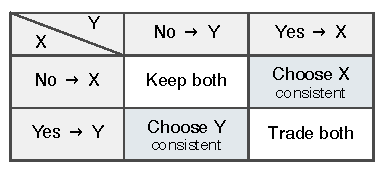
\includegraphics[width=0.64\textwidth]{task_overview.pdf}
\caption{Paired response map. $X$ indexes the X-endowed response and $Y$
indexes the Y-endowed response. The shaded off-diagonal cells select the same
final good under both endowments. The diagonal cells keep or trade both and
therefore depend on ownership.}
\label{fig:task}
\end{figure}

Figure~\ref{fig:task} shows why a constant answer is not ownership-neutral.
Always answering ``No'' produces keep-both: the model chooses $X$ when it owns
$X$ and $Y$ when it owns $Y$. Always answering ``Yes'' produces trade-both and
also reverses the selected good when the endowment changes. Ownership-invariant
choice occupies the off-diagonal cells.

\subsection{Structural measurement}

\subsubsection{Preference and utility interpretation}

We treat a model as a decision-maker with an agent-specific latent preference
relation over the finite set of good--attribute configurations. The working
assumption is that this relation is stable over the elicitation and training
window. Stability is a modeling restriction in the tradition of treating
tastes as fixed \citep{stigler1977degustibus}, not an empirical fact guaranteed
for language models: behavioral work shows that expressed preferences can be
constructed by framing and context \citep{slovic1995construction}. We therefore
test the fitted ordering against separate ownership-free prompts rather than
equating any single elicitation with preference itself.

If the within-agent relation is complete and transitive, it admits a numerical
utility representation \citep{debreu1954representation}. For this finite task,
``global'' means that one fitted ordering covers every configuration in the
benchmark for that model. It does not mean a universal ranking shared by
people or models, and it has no social-welfare interpretation. The numerical
representation is ordinal absent additional structure: its sign comparisons
encode the ranking, whereas distances require a chosen scale and functional
form.

Our chosen structure follows characteristics-based consumer modeling
\citep{lancaster1966new}: a configuration $g=(m,a)$ combines item identity $m$
with a generic attribute profile $a=(a_1,a_2)$. Define the latent index and
positive utility score as
\begin{equation}
v_g=\alpha_m+\beta_a,
\qquad
U_g=\exp(v_g).
\label{eq:configuration-utility}
\end{equation}
The first item and attribute profile $(1,1)$ are reference categories, so
$\alpha_1=\beta_{1,1}=0$ and their reference score is one. The exponential
ensures positivity but is a parametric normalization, not evidence that
$U_g$ is intrinsically cardinal.

\subsubsection{Reference-dependent choice model}

Observed endowed choices combine this fitted configuration score with an
ownership-dependent term. For the X-endowed prompt, the latent keep-versus-
trade score is
\begin{equation}
z_i^X=(1+\lambda)U_{X_i}-U_{Y_i}+\eta,
\label{eq:structural}
\end{equation}
and the Y-endowed equation swaps $X$ and $Y$. A logistic link maps the score to
the probability of keeping the endowed good. This separates a stable
configuration component from reference-dependent choice, following the
behavioral distinction between consumption value and changes induced by the
reference state \citep{tversky1991loss}. The multiplier $1+\lambda$ captures
ownership-specific asymmetry, while $\eta$ captures a general status-quo
tendency. This particular multiplier is our task-specific structural
parameterization, not the canonical prospect-theory value function. The
ownership-neutral target is $(\lambda,\eta)=(0,0)$, but the parameters must be
interpreted jointly: a small $\lambda$ can coexist with substantial rigidity
absorbed by $\eta$.

\begin{table}[htbp]
\centering
\small
\begin{tabular}{p{0.18\textwidth}p{0.72\textwidth}}
\toprule
Quantity & Interpretation \\
\midrule
$\widehat\lambda$ & Structural ownership asymmetry under the endowed-good multiplier $1+\lambda$. \\
$\widehat\eta$ & General tendency to preserve the status quo, independent of which good is endowed. \\
Consistency & Fraction of paired configurations that select the same final good under both endowments. \\
Keep-both & Fraction with $(\text{No},\text{No})$; chooses whichever good is endowed. \\
Trade-both & Fraction with $(\text{Yes},\text{Yes})$; chooses whichever good is not endowed. \\
$W$ & Mean pseudo-utility alignment $u_{\mathrm{chosen}}/\max(u_X,u_Y)$ against one shared positive Qwen reference; descriptive and ID-only. \\
Higher-utility choice & Fraction of endowed-task choices that select the good with higher shared reference utility; distinct from a separate ownership-free prompt. \\
Preference agreement & Agreement of a trained policy with frozen ownership-free preferences; this remains pending and is distinct from reward-signal validation. \\
\bottomrule
\end{tabular}
\caption{Structural and direct outcomes reported together.}
\label{tab:metrics}
\end{table}

% =============================================================================
\section{Data and Split Roles}

The original benchmark contains 59,400 paired configurations and 118,800
perspective-specific prompts over 100 goods and all 4,950 unordered goods
pairs. Five pairs supply 60 trial configurations. The remaining 4,945 pairs
appear in both training and configuration validation, with disjoint attribute
profiles.

\begin{table}[htbp]
\centering
\small
\begin{tabular}{lrrrrp{0.26\textwidth}}
\toprule
Split & Goods & Pairs & Configurations & Prompts & Role \\
\midrule
Trial & 6 & 5 & 60 & 120 & Sanity checks. \\
Training & 100 & 4,945 & 49,450 & 98,900 & Ten configurations per pair; used by GRPO. \\
Configuration validation & 100 & 4,945 & 9,890 & 19,780 & Two disjoint configurations per pair; used for checkpoint selection. \\
Frozen OOD-50 & 50 new & 1,225 & 9,800 & 19,600 & Eight configurations per pair; new goods and categories. \\
\bottomrule
\end{tabular}
\caption{Dataset roles. OOD-50 is a separate evaluation suite and is not part
of the 59,400-configuration original benchmark.}
\label{tab:data}
\end{table}

Training and configuration validation contain zero repeated exact
configurations and zero repeated prompt strings. They nevertheless share the
same 100 goods and 4,945 pair identities, so the narrow interpretation is
generalization to unseen attribute configurations of familiar goods and pairs.
For the Qwen-derived run, \texttt{test\_goods} is validation rather than an
untouched final test: responses from this split informed the fitted
pseudo-utility and seven checkpoint estimates were inspected before selecting
step 8,000.

The OOD suite was generated with seed 20260710 and contains 50 new goods in 10
new categories, 100 new attribute names, and 1,225 unordered pairs. Category
names, good names, attribute names, and complete attribute-value strings have
zero exact overlap with the original catalogue. It was excluded from reward
construction, training, and exploratory checkpoint selection. For every OOD
comparison, the correct base comparator is the base evaluated on OOD-50, not
the ID base.

% =============================================================================
\section{Qwen-Derived Pseudo-Utility and Reward}

\subsection{Utility recovery from paired probabilistic choices}

The primary reference was estimated once from the historical Together-hosted
Qwen endpoint and then frozen during GRPO. It is not recomputed by the exact
local base, the current adapter, or any later checkpoint. Each comparison
supplies two observations: one with $X$ endowed
and one with $Y$ endowed. For each prompt, the outcome
$q_{i,p}^{\mathrm{keep}}$ is the normalized model probability of ``No,'' since
``No'' keeps the endowed good. In the historical reward-source fit these were
normalized top-five first-token probabilities; the matched local evaluation
instead uses exact teacher-forced sequence scores. The common structural link
scale is fixed at $T=1$.

Model A jointly estimates $\lambda$, $\eta$, 99 non-reference item effects,
and eight non-reference attribute-profile effects by nonlinear least squares:
\begin{equation}
\widehat\theta
=\arg\min_\theta
\sum_{i,p\in\{X,Y\}}
\left[q_{i,p}^{\mathrm{keep}}-
\sigma\!\left(z_{i,p}(\theta)/T\right)\right]^2,
\qquad T=1.
\label{eq:nls-utility}
\end{equation}
The two counterfactual endowments provide the variation used to separate the
configuration scores $U_g$ from $\lambda$ and $\eta$. This is a parametric
random-utility-style interpretation of probabilistic discrete choice
\citep{mcfadden2000economic,train2009discrete}; the fitted $U_g$ are not
directly observed tastes. They are identified only relative to the reference
categories, fixed link scale, exponential specification, and the assumption
that ownership enters through Equation~\ref{eq:structural}.

After fitting, Equation~\ref{eq:configuration-utility} yields one positive
score for each of the $100\times9=900$ item--profile configurations. The
ownership-neutral comparison used by training removes the fitted ownership and
status-quo terms:
\begin{equation}
\dd_i=\widehat U_{X_i}-\widehat U_{Y_i}.
\label{eq:pseudo-delta}
\end{equation}
Thus $\operatorname{sign}(\dd_i)$ is the historical endpoint's fitted ranking, while
$|\dd_i|$ is a model-scale separation weight. A strictly
increasing transformation would preserve the sign but generally change the
magnitude, which is why we call the values pseudo-utilities and retain a
sign-only GRPO baseline as an important robustness test.

The safest provenance description is \emph{historical-Qwen-derived}. The
pseudo-utility was fitted from the historical
Together-hosted Qwen2.5-7B-Instruct-Turbo evaluation, while the ownership-free
anchors used below were elicited from the exact local Qwen2.5-7B-Instruct
weights. The artifacts therefore do not yet establish that the reward is the
exact tuned checkpoint's own frozen ordering.

\subsection{Reward direction}

The primary training signal uses the fitted difference in
Equation~\ref{eq:pseudo-delta}. If $\dd_i>0$, the target is to select $X$:
answer ``No'' when endowed with $X$
and ``Yes'' when endowed with $Y$. The mapping reverses when $\dd_i<0$. If
$r_i^\star$ is the target response, the reward is
\begin{equation}
\mathcal R(\widehat r_i,\dd_i)=
\begin{cases}
+|\dd_i|,&\widehat r_i=r_i^\star,\\
-|\dd_i|,&\text{otherwise}.
\end{cases}
\label{eq:reward}
\end{equation}
In a mixed-response group, an unparseable output is treated as incorrect and
receives the negative reward. If all 16 parsed outputs are identical, including
an all-unparseable group, the implementation returns zero for the entire group
and skips the update. Magnitude weighting assigns the strongest updates to
comparisons for which the fitted ordering is most decisive.

\subsection{Identification and cross-elicitation validation}

The historical endowed evaluator answers ``No'' almost all the time, but its
utility fit uses continuous normalized Yes/No probabilities recovered from
historical top-five first-token log probabilities at structural link scale
$T=1$, not only hard answers. Two prompts can decode to ``No'' while assigning
meaningfully different probability to ``Yes.'' The resulting fixed effects and
utility differences remain dispersed and statistically identified.

\begin{table}[htbp]
\centering
\small
\begin{tabular}{p{0.34\textwidth}p{0.56\textwidth}}
\toprule
Diagnostic & Observed value \\
\midrule
Item effects $\alpha$ & 99/99 with non-zero SE; median $|t|=9.6$; 91.9\% significant. \\
Attribute effects $\beta$ & 8/8 with non-zero SE; median $|t|=27.5$; 100\% significant. \\
Pseudo-utility spread & SD $0.94$; range $[-4.06,3.91]$; 1.6\% near zero; 46.9\% positive. \\
Stable ownership-free anchors & 6,184/9,890 validation and 30,757/49,450 training configurations. \\
\bottomrule
\end{tabular}
\caption{Identification diagnostics for the Qwen-derived pseudo-utility.}
\label{tab:delta-identification}
\end{table}

Ownership-free preferences were elicited with two paraphrases and both display
orders. A case is retained only when the elicitation is sufficiently stable.
The comparison is convergent evidence across Qwen-family endpoints and
elicitation frames; it is not independent human ground truth.

\begin{table}[htbp]
\centering
\small
\begin{tabular}{lrrr}
\toprule
Split & Stable cases & Overall agreement & Agreement for $|\dd|>1$ \\
\midrule
Configuration validation & 6,184 & 71.1\% & 85.5\% \\
Training & 30,757 & 70.8\% & 85.3\% \\
\bottomrule
\end{tabular}
\caption{Agreement between $\operatorname{sign}(\dd)$ and stable
ownership-free Qwen choices. This validates the reward direction, not the
trained policy.}
\label{tab:anchor}
\end{table}

\begin{table}[htbp]
\centering
\small
\begin{tabular}{lrr}
\toprule
Magnitude band & Validation agreement & Training agreement \\
\midrule
$|\dd|\leq0.5$ & 63.6\% & 62.3\% \\
$0.5<|\dd|\leq1.0$ & 67.9\% & 70.0\% \\
$|\dd|>1.0$ & 85.5\% & 85.3\% \\
\bottomrule
\end{tabular}
\caption{Reward-direction agreement increases with pseudo-utility magnitude,
which is also the reward weight in Equation~\ref{eq:reward}.}
\label{tab:anchor-magnitude}
\end{table}

\FloatBarrier
\subsection{Frontier-consensus reward-source ablation}

The reward-source ablation averages fitted utility differences from six
frontier systems: GPT-4o, GPT-5, GPT-5.2, Gemini 1.5 Pro, Llama-70B, and
DeepSeek-R1. The six systems agree on the sign for about 64\% of all 59,400
configurations; otherwise their mean typically supplies a lower-magnitude target. This
signal is also a pseudo-utility, not objective cardinal truth. Its role is to
show what changes when the reward source is an external model consensus rather
than Qwen-derived. Because utility scales are model-dependent, this average is
an operational aggregation rule over fitted scores, not a theoretically unique
population preference or an interpersonal welfare comparison.

% =============================================================================
\section{Training Procedure}

The model is Qwen2.5-7B-Instruct \citep{qwen2024qwen25}. Training updates LoRA
adapters \citep{hu2021lora} with GRPO \citep{shao2024deepseekmath}. For each
prompt, 16 completions are sampled, scored with Equation~\ref{eq:reward}, and
compared within the group. Groups with no reward variation produce no useful
relative advantage and are filtered. This DAPO-style behavior
\citep{yu2025dapo} avoids invalid updates but does not avoid the generation
cost of all-identical groups.

\begin{table}[htbp]
\centering
\small
\begin{tabular}{L{0.20\textwidth}L{0.31\textwidth}L{0.39\textwidth}}
\toprule
Component & Setting & Notes \\
\midrule
Base model & Qwen2.5-7B-Instruct & Local Hugging Face weights. \\
Adapter & LoRA rank 16, $\alpha=32$, dropout 0.05 & Attention and MLP projections. \\
Group size & 16 & Completions per prompt. \\
Rollout temperature & 1.5 & Increases output diversity. \\
Learning rate & $10^{-6}$ & Conservative update. \\
Clip parameter & 0.2 & Policy-ratio clipping. \\
KL coefficient & 0.04 & Keeps the adapter near the base policy. \\
Completion length & 4 tokens & Sufficient for Yes/No output. \\
Loss and scaling & DAPO; no reward scaling & Zero-variance groups carry no update. \\
Effective batch & batch 1, accumulation 16 & One A100-40GB. \\
Precision & bfloat16 & Plain Hugging Face path; no working vLLM dependency. \\
Exploratory seed & 42 & Inferred from the original default. \\
\bottomrule
\end{tabular}
\caption{Training configuration used for the completed exploratory run.}
\label{tab:hyperparameters}
\end{table}

The working NSCC path uses plain Hugging Face generation because compatible
vLLM builds failed in the cluster environment. Training was made resumable
across 72-hour PBS jobs with checkpoints every 200 steps. Monitoring later
showed a high fraction of zero-variance groups and non-monotonic structural
performance; consequently, training reward is treated as a diagnostic rather
than the model-selection outcome.

The original training program did not explicitly pass a seed, so the completed
run used the library default, seed 42. Seed handling has since been added to the
CLI, configuration, GRPO arguments, output directories, and logs. Confirmatory
seeds 1 and 2 will therefore measure independent training variation rather
than silent reuse of the same random stream.

% =============================================================================
\section{Evaluation and Checkpoint Selection}

\subsection{Scoring and estimation}

Evaluation greedily generates a hard answer for direct choice counts and also
computes exact normalized teacher-forced sequence scores for ``Yes'' and
``No'' from the native logits:
\begin{equation}
P_\theta(\text{Yes}\mid x,\{\text{Yes},\text{No}\})=
\frac{\exp(s_{\text{Yes}})}
{\exp(s_{\text{Yes}})+\exp(s_{\text{No}})},
\quad
s_a=\sum_t\log p_\theta(a_t\mid x,a_{<t}).
\end{equation}
These deterministic probabilities are passed to Model A nonlinear least
squares at link scale $T=1$. A prior $T=0$ run caused a silent zero-Jacobian
failure, so finite non-zero standard errors are now mandatory. Current
structural standard errors remain conditional NLS errors; they do not yet
capture repeated pairs, shared goods, or training-seed variation.

\subsection{Exploratory checkpoint sweep}

Seven checkpoints from the completed seed-42 run were evaluated on
\texttt{test\_goods}. Step 8,000 was chosen after examining both $\lambda$ and
$\eta$, making the result retrospective. A joint rule was later frozen for new
seeds: retain checkpoints with consistency at least 0.50 and finite non-zero
standard errors, then minimize
\begin{equation}
d=\sqrt{\widehat\lambda^2+\widehat\eta^2},
\end{equation}
If two distances differ by less than $0.05$, the higher-consistency checkpoint
is preferred; if consistency then differs by less than $0.02$, the earlier
checkpoint is selected.

\begin{figure}[htbp]
\centering
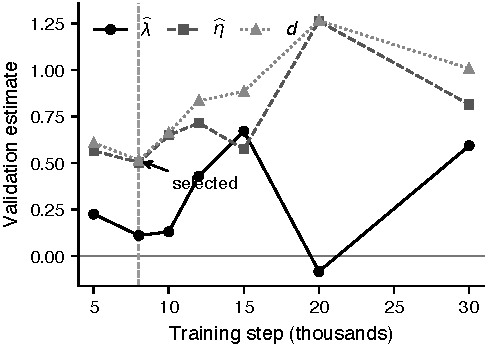
\includegraphics[width=0.56\textwidth]{checkpoint_curve.pdf}
\caption{Exploratory seed-42 validation curve. The structural estimates are
non-monotonic; step 8,000 has the smallest joint distance $d$ among the seven
observed checkpoints. The rule was frozen only after these results were known.}
\label{fig:checkpoint}
\end{figure}

\begin{table}[htbp]
\centering
\small
\begin{tabular}{rrrrrr}
\toprule
Step & $\widehat\lambda$ & $\widehat\eta$ & Consistency & $d$ & Reading \\
\midrule
5,000  & 0.226 & 0.566 & 60.98\% & 0.609 & eligible \\
8,000  & 0.111 & 0.504 & 69.68\% & 0.516 & selected \\
10,000 & 0.131 & 0.650 & 71.06\% & 0.663 & eligible \\
12,000 & 0.430 & 0.717 & 65.74\% & 0.836 & eligible \\
15,000 & 0.673 & 0.576 & 65.14\% & 0.886 & eligible \\
20,000 & $-0.083$ & 1.263 & 76.91\% & 1.266 & small $|\lambda|$, large $\eta$ \\
30,000 & 0.593 & 0.815 & 72.81\% & 1.008 & eligible \\
\bottomrule
\end{tabular}
\caption{Full checkpoint grid evaluated for the exploratory seed-42 run.}
\label{tab:checkpoints}
\end{table}

For confirmatory seeds, the grid was fixed at every 2,000 steps from 2,000 to
30,000. Selection used ID validation only, and OOD-50 was opened once after
selection at the chosen checkpoint. Seed 1 selected step 2,000 and seed 2
selected step 6,000. Both passed the frozen rule, so no third seed was required.
Seed 42 remains excluded from the confirmatory denominator.

% =============================================================================
\section{Results Completed So Far}

\subsection{Why the historical base was replaced}

The original baseline used a Together-hosted Turbo endpoint, 9,950 cases, and
top-five first-token probabilities. The matched base uses the exact local
weights, the same 9,890 rows, the same teacher-forced sequence scorer, and the
same estimator as the tuned models. The historical value is retained only as a
measurement-history note.

\begin{table}[htbp]
\centering
\small
\begin{tabular}{lrrrrp{0.28\textwidth}}
\toprule
Base evaluation & $N$ & $\widehat\lambda$ & SE & $\widehat\eta$ & Why it is used \\
\midrule
Historical Together Turbo & 9,950 & 11.752 & 1.222 & 1.518 & Superseded; endpoint and scorer mismatch. \\
Exact local matched base & 9,890 & 7.637 & 0.627 & 1.007 & Comparator for every ID before/after statement. \\
\bottomrule
\end{tabular}
\caption{The historical baseline is about 54\% larger than the matched local
estimate, illustrating why pipeline matching matters.}
\label{tab:base-history}
\end{table}

\subsection{Configuration-validation results}

\begin{table}[htbp]
\centering
\scriptsize
\begin{tabular}{lrrrrrrr}
\toprule
Model & $\widehat\lambda$ & $\widehat\eta$ & $W$ & Cons. & Keep & Trade & Pref. agr. \\
\midrule
Exact local base & 7.637 & 1.007 & 0.744 & 0.87\% & 99.13\% & 0.00\% & -- \\
Qwen-derived SFT & -- & -- & -- & -- & -- & -- & -- \\
Qwen-derived GRPO seed 1, step 2k & 0.032 & 0.091 & 0.883 & 66.15\% & 18.24\% & 15.61\% & -- \\
Qwen-derived GRPO seed 2, step 6k & $-0.042$ & 0.659 & 0.910 & 71.76\% & 20.98\% & 7.26\% & -- \\
Qwen-derived GRPO seed 42 (exploratory) & 0.111 & 0.504 & 0.909 & 69.68\% & 24.17\% & 6.16\% & -- \\
Consensus GRPO ablation & 0.177 & $-0.048$ & 0.890 & 90.65\% & 7.84\% & 1.30\% & -- \\
\bottomrule
\end{tabular}
\caption{Matched results on the 9,890 configuration-validation cases. The
post-training rows are validation-only. $W$ uses one shared historical Qwen
utility reference and was added after the seed pre-registration. Preference
agreement for the trained policies remains pending; the 71.1\% reward-signal
validation is not inserted into that column.}
\label{tab:id-results}
\end{table}

\begin{table}[htbp]
\centering
\small
\begin{tabular}{lrrr}
\toprule
Model & $\widehat\lambda$ (SE) & $\widehat\eta$ (SE) & Higher-utility choice \\
\midrule
Exact local base & 7.637 (0.627) & 1.007 (0.120) & 50.42\% \\
Qwen-derived GRPO seed 1, step 2k & 0.032 (0.015) & 0.091 (0.031) & 71.23\% \\
Qwen-derived GRPO seed 2, step 6k & $-0.042$ (0.012) & 0.659 (0.029) & 75.51\% \\
Qwen-derived GRPO seed 42 & 0.111 (0.014) & 0.504 (0.029) & 75.29\% \\
Consensus GRPO ablation & 0.177 (0.005) & $-0.048$ (0.024) & 72.48\% \\
\bottomrule
\end{tabular}
\caption{ID structural uncertainty and reference-choice summary for completed
rows. Higher-utility choice is measured within the endowed task against the
shared Qwen-derived utility table; it is not the pending ownership-free prompt
agreement experiment.}
\label{tab:id-se-rational}
\end{table}

Under the matched pipeline, the exploratory Qwen-derived model has a much
smaller $\widehat\lambda$ than the exact local base, while
$\widehat\eta=0.504$ and a 24.17\% keep-both rate show residual status-quo
rigidity. The consensus ablation has a somewhat larger $\widehat\lambda$ but
near-zero $\widehat\eta$ and 90.65\% consistency. The reward sources therefore
trade off rather than dominate one another.

\subsection{Frozen new-goods results}

\begin{table}[htbp]
\centering
\scriptsize
\begin{tabular}{lrrrrrr}
\toprule
Model & $\widehat\lambda$ & SE & $\widehat\eta$ & SE & Cons. & Keep / Trade \\
\midrule
Exact local base & 2.209 & 0.261 & 5.358 & 0.081 & 0.04\% & 99.96\% / 0.00\% \\
Qwen-derived SFT & -- & -- & -- & -- & -- & -- \\
Qwen-derived GRPO seed 1, step 2k & 0.259 & 0.023 & 0.323 & 0.035 & 50.44\% & 38.71\% / 10.85\% \\
Qwen-derived GRPO seed 2, step 6k & 0.064 & 0.016 & 0.593 & 0.034 & 59.83\% & 31.10\% / 9.07\% \\
Qwen-derived GRPO seed 42 (exploratory) & 0.226 & 0.020 & 0.790 & 0.038 & 49.46\% & 46.01\% / 4.53\% \\
Consensus GRPO ablation & 0.395 & 0.018 & 0.502 & 0.043 & 64.89\% & 34.74\% / 0.37\% \\
\bottomrule
\end{tabular}
\caption{OOD-50 results for the exploratory, confirmatory, and reward-source
models. Every trained model is compared with the OOD base, never with the ID
base. Raw OOD predictions are not yet included in the cloneable repository.}
\label{tab:ood-results}
\end{table}

The exact OOD base is almost completely endowment-locked and has a very large
$\widehat\eta$. Both confirmatory seeds pass the pre-registered OOD and
non-degeneracy gates. The exploratory Qwen-derived model has lower
$\widehat\lambda$ than the consensus ablation, while the consensus ablation
has lower $\widehat\eta$ and higher consistency. Seed 42's OOD consistency is
49.46\%, 0.54 percentage points below the 0.50 no-degeneracy floor later
pre-registered for new seeds. That criterion does not retroactively grade the
exploratory run, but the proximity should be reported rather than hidden.

\subsection{Frozen prospective unused-configuration results}

After checkpoint selection and the OOD-50/GSM8K verdict were complete, a
prospective suite reserved 10 previously unused attribute configurations for
each of the 4,945 familiar goods pairs. It was opened once for the matched base
and the two selected confirmatory checkpoints. This is a within-benchmark
configuration test, not an unseen-goods test.

\begin{table}[htbp]
\centering
\small
\begin{tabular}{lrrrrrr}
\toprule
Model & $\widehat\lambda$ & SE & $\widehat\eta$ & SE & Cons. & $W$ \\
\midrule
Exact local base & 5.946 & 0.192 & 1.458 & 0.046 & 0.76\% & 0.742 \\
Seed 1, step 2k & 0.031 & 0.007 & 0.089 & 0.014 & 65.92\% & 0.882 \\
Seed 2, step 6k & $-0.053$ & 0.005 & 0.693 & 0.013 & 71.61\% & 0.909 \\
\bottomrule
\end{tabular}
\caption{Once-opened prospective results on 49,450 unused configurations of
familiar goods and pairs. The result supports configuration generalization but
does not replace the separate new-goods OOD-50 evaluation.}
\label{tab:frozen-unused}
\end{table}

\subsection{Pseudo-utility alignment distribution}

For ID cases only, $W$ measures the chosen good's positive reference utility
as a fraction of the better available reference utility. A choice of the
higher-utility good has $w=1$. OOD goods do not occur in the shared historical
reference and therefore do not receive comparable $W$ values.

\begin{table}[htbp]
\centering
\small
\begin{tabular}{lrrr}
\toprule
$w$ range & Local base & Qwen-derived 8k & Consensus ablation \\
\midrule
$0.0\leq w<0.2$ & 8.43\% & 0.83\% & 1.17\% \\
$0.2\leq w<0.4$ & 13.40\% & 4.01\% & 5.67\% \\
$0.4\leq w<0.6$ & 10.71\% & 5.82\% & 6.75\% \\
$0.6\leq w<0.8$ & 9.18\% & 6.69\% & 6.70\% \\
$0.8\leq w<1.0$ & 7.85\% & 7.35\% & 7.22\% \\
$w=1$ & 50.42\% & 75.29\% & 72.48\% \\
\bottomrule
\end{tabular}
\caption{Distribution of the descriptive ID pseudo-utility alignment score.}
\label{tab:w-distribution}
\end{table}

% =============================================================================
\section{Additional Diagnostics}

\subsection{Attribute-configuration sensitivity}

The completed attribute analysis uses the \emph{consensus-delta policy's}
baseline-treatment responses. It establishes that the reserved attribute
configurations are behaviorally consequential for that trained policy; it
should not be presented as a Qwen-derived seed-42-specific diagnostic without
rerunning the script on that model's raw predictions.

\begin{table}[htbp]
\centering
\small
\begin{tabular}{p{0.58\textwidth}r}
\toprule
Diagnostic & Result \\
\midrule
Differenced observations / pair clusters & 9,890 / 4,945 \\
Pair-clustered joint test & $\chi^2(8)=5{,}097.22$, $p<10^{-1000}$ \\
Leave-one-good-out joint test & $\chi^2(8)=756.05$, $p<10^{-150}$ \\
Within-pair, within-perspective $R^2$ & 0.488 \\
Mean absolute change in $P(\mathrm{No})$ & 0.340 \\
X / Y answer flips & 34.07\% / 34.24\% \\
At least one / both perspectives flip & 42.18\% / 26.13\% \\
Pair-grouped CV MSE reduction from attributes & 47.43\% \\
\bottomrule
\end{tabular}
\caption{Held-out attribute-configuration diagnostics for the consensus-delta
policy.}
\label{tab:attribute-summary}
\end{table}

The eight generic $3\times3$ ordinal profiles are estimated relative to
$(1,1)$. These coefficients are probability diagnostics, not the structural
utility $\beta$ coefficients and not distinct semantic attributes such as
flavor or scent.

\begin{table}[htbp]
\centering
\small
\begin{tabular}{lrrr}
\toprule
Profile & Effect on $P(\mathrm{No})$ & Pair-clustered SE & Leave-one-good-out SE \\
\midrule
$(1,2)$ & 0.177 & 0.011 & 0.016 \\
$(1,3)$ & 0.298 & 0.011 & 0.016 \\
$(2,1)$ & 0.228 & 0.011 & 0.017 \\
$(2,2)$ & 0.446 & 0.011 & 0.021 \\
$(2,3)$ & 0.546 & 0.011 & 0.022 \\
$(3,1)$ & 0.355 & 0.011 & 0.020 \\
$(3,2)$ & 0.566 & 0.011 & 0.025 \\
$(3,3)$ & 0.630 & 0.011 & 0.024 \\
\bottomrule
\end{tabular}
\caption{Full ordinal-profile sensitivity table for the consensus-delta
policy.}
\label{tab:attribute-profiles}
\end{table}

\subsection{Prompt-treatment robustness for the consensus adapter}

Earlier evaluations varied the prompt while keeping the consensus-trained
adapter fixed. The debias prompt explicitly asks the model to ignore status
quo and gain/loss attitudes. The forced prompt says that a kept good still has
a 50\% probability of being switched. These are secondary prompt-robustness
results, not evidence about the primary Qwen-derived model.

\begin{table}[htbp]
\centering
\small
\begin{tabular}{lrrrrrr}
\toprule
Prompt treatment & $\widehat\lambda$ & SE & $\widehat\eta$ & SE & Cons. & Keep / Trade \\
\midrule
Baseline wording & 0.177 & 0.005 & $-0.048$ & 0.024 & 90.65\% & 7.84\% / 1.30\% \\
Debias instruction & 0.205 & 0.005 & 0.090 & 0.024 & 88.77\% & 10.18\% / 0.76\% \\
Forced random switch & 0.173 & 0.006 & $-0.379$ & 0.022 & 89.26\% & 5.36\% / 4.92\% \\
\bottomrule
\end{tabular}
\caption{Secondary prompt-treatment results for the consensus-delta adapter.}
\label{tab:treatments}
\end{table}

\FloatBarrier
% =============================================================================
\section{Capability Retention}

GSM8K \citep{cobbe2021gsm8k} was run on all 1,319 test questions with 8-shot
chain-of-thought prompting, greedy decoding, and 100\% answer parsing for both
models. The comparison is paired by question.

\begin{table}[htbp]
\centering
\small
\begin{tabular}{lrr}
\toprule
Model & Correct & Accuracy \\
\midrule
Exact local base & 1,146 / 1,319 & 86.88\% \\
Qwen-derived GRPO seed 42, step 8k & 1,133 / 1,319 & 85.90\% \\
\bottomrule
\end{tabular}
\caption{Completed GSM8K capability check. The tuned-minus-base change is
$-0.99$ percentage points; paired bootstrap 95\% CI
$[-2.12,+0.15]$; exact McNemar $p=0.111$.}
\label{tab:gsm8k}
\end{table}

There are 35 base-only correct questions and 22 tuned-only correct questions.
The interval spans zero, so the current reading is ``no clear statistically
significant change,'' not capability equivalence or identical performance.
IFEval \citep{zhou2023ifeval} remains pending, as does the capability check for
the SFT baseline. Confirmatory seed 1 changes GSM8K accuracy by $-0.15$
percentage points (95\% CI $[-1.14,+0.83]$), and seed 2 by $-0.30$ points
(95\% CI $[-1.44,+0.83]$); both pass the frozen $-3$ point lower-bound gate.

\FloatBarrier
% =============================================================================
\section{Reproducibility and Artifact Status}

The repository contains the training and evaluation programs, exact
configurations, checkpoint rule, pre-registration, structural result CSVs,
choice-count tables, Qwen-anchor validation, GSM8K summaries, and per-result
manifests with checksums and reproduction commands. The exact-local-base and
primary ID raw X/Y prediction files are tracked in the current repository.

The cloneable record is still incomplete. OOD raw X/Y predictions are absent,
selected adapter weights are represented by hashes rather than distributable
files, and the GSM8K item-level prediction JSONL files are not present. Thus,
the derived results are traceable, but a fresh clone cannot yet reproduce every
claim from raw model outputs.

\begin{table}[htbp]
\centering
\small
\begin{tabular}{p{0.36\textwidth}p{0.18\textwidth}p{0.36\textwidth}}
\toprule
Artifact group & Status & Remaining action \\
\midrule
Training/evaluation code and configs & Available & Freeze environment and version record. \\
Checkpoint-selection protocol and pre-registration & Applied & Frozen rule applied unchanged to seeds 1 and 2. \\
Matched-base and primary-ID raw predictions & Tracked & Verify anonymous package paths and checksums. \\
Derived ID/OOD/GSM8K estimates and manifests & Tracked & Keep commands synchronized with final code. \\
OOD raw predictions & Missing from clone & Archive in anonymous supplement or external dataset. \\
Selected adapters & Hashes only & Archive distributable weights or document controlled access. \\
GSM8K item predictions & Missing from clone & Add anonymized JSONL outputs. \\
Environment lock & Partial & Record Python, PyTorch, TRL, Transformers, PEFT, and CUDA versions. \\
\bottomrule
\end{tabular}
\caption{Current reproducibility-package status.}
\label{tab:artifacts}
\end{table}

Key reproduction entry points include:
\begin{itemize}
    \item matched local base: \texttt{qsub train/submit\_eval\_base\_matched.pbs};
    \item exploratory checkpoint evaluation: \texttt{qsub -v CKPT=8000 train/submit\_eval\_ckpt.pbs};
    \item checkpoint selection: \texttt{python eval/select\_checkpoint.py};
    \item OOD evaluation: \texttt{qsub train/submit\_eval\_ood\_new\_goods.pbs};
    \item Qwen-anchor validation: \texttt{python eval/validate\_qwen\_delta\_anchor.py}; and
    \item attribute diagnostics: \texttt{python eval/analyze\_attribute\_effects.py}.
\end{itemize}

\FloatBarrier
% =============================================================================
\section{Work Still in Progress}

\begin{table}[!htbp]
\centering
\small
\begin{tabular}{p{0.28\textwidth}p{0.18\textwidth}p{0.44\textwidth}}
\toprule
Work item & Priority & What it answers \\
\midrule
Matched Qwen-derived SFT & Required & Are binary supervised targets sufficient without GRPO? \\
Pair-cluster bootstrap & Required & How sensitive are $\lambda$ and $\eta$ intervals to paired dependence? \\
Leave-one-good-out structural inference & Required & Do the structural estimates depend on a small number of goods? \\
Estimator-recovery simulation & Required & Can Model A recover known $\lambda$ and $\eta$ under the benchmark design? \\
IFEval & Required & Is instruction following retained alongside GSM8K? \\
Trained-policy preference agreement & Required & Does the final policy preserve the frozen ownership-free ordering? \\
OOD raw/archive completion & Required & Can a reviewer independently regenerate the OOD tables? \\
Sign-only GRPO & Optional & Does pseudo-utility magnitude add value beyond the target sign? \\
Human anchor subset & Optional & Does the Qwen-derived ordering agree with an external preference source? \\
\bottomrule
\end{tabular}
\caption{Unfinished experiments and the questions they address.}
\label{tab:pending}
\end{table}

Both confirmatory seeds passed the pre-registered requirements:
$|\widehat\lambda|\leq0.5$, consistency at least 0.50, keep-both and trade-both
at most 0.50, and a paired GSM8K interval lower bound of at least $-3$
percentage points. $\eta$ was reported but not gated; the project
pre-declared that it would not claim $\eta$ is eliminated.

\FloatBarrier
% =============================================================================
\section{Current Interpretation, Limitations, and Non-Claims}

The project has established an end-to-end intervention and evaluation
pipeline. One exploratory and two confirmatory Qwen-derived GRPO adapters move
the structural ownership-asymmetry estimate far toward zero under matched
ID pipelines and retain low estimates on the frozen new-goods suite. The two
selected confirmatory adapters also produce near-zero $\lambda$ on the
prospective unused-configuration suite. The project has also
shown that the reward source matters: the Qwen-derived and consensus rewards
occupy different points in the joint space of $\lambda$, $\eta$, consistency,
and pseudo-utility alignment.

The evidence does not yet establish that GRPO is necessary because the matched
SFT comparison is unfinished. Training reliability is supported by two
confirmatory seeds that pass the frozen rule, but all seed-level outcomes must
be reported jointly. The seed-42 ID result remains validation-only, and the
OOD evidence is not fully reproducible until its raw artifacts are archived.
Conditional NLS errors do not
replace pair-aware, good-aware, and seed-level uncertainty. The Qwen-derived
reward is a cross-endpoint model-family signal rather than objective cardinal
ground truth.

We therefore do not claim:
\begin{itemize}
    \item that loss aversion or status-quo bias is completely eliminated;
    \item that the model is superior to humans or every frontier model;
    \item that the commonly cited human coefficient is directly comparable to
          this task's $1+\lambda$ parameterization;
    \item that \texttt{test\_goods} is an untouched final test;
    \item that Qwen-derived reward dominates consensus reward on every metric;
    \item that GSM8K proves capability equivalence; or
    \item that the current results establish GRPO's advantage over SFT.
\end{itemize}

The narrow conclusion is descriptive: the implemented Qwen-derived GRPO
intervention substantially changes ownership-dependent choice in one
exploratory run and generalizes partially to new goods. GSM8K shows no clear
statistically significant change under the current paired comparison. The next phase determines
whether those observations replicate, whether GRPO adds value over supervised
training, and whether the structural and capability conclusions survive more
appropriate uncertainty estimates.

\clearpage
% =============================================================================
\section{Short Project Record}

\begin{table}[htbp]
\centering
\small
\begin{tabular}{lp{0.72\textwidth}}
\toprule
Period & Work completed \\
\midrule
April 2026 & Inherited endowment-effect evaluator; established historical Qwen baseline; implemented consensus pseudo-utility and GRPO reward. \\
April--June 2026 & Built resumable NSCC training, LoRA/GRPO configuration, reward filtering, and a stable plain-Hugging-Face training path. \\
June 2026 & Added vLLM-free local sequence scoring and structural evaluation. \\
Early July 2026 & Completed consensus-delta evaluation and baseline/debias/forced prompt treatments. \\
Mid July 2026 & Selected Qwen-derived step 8,000 as the primary exploratory model; completed matched local base, OOD-50 evaluation, pseudo-utility validation, checkpoint protocol, seed pre-registration, GSM8K, manifests, and pseudo-utility alignment. \\
Late July 2026 & Confirmatory seeds 1 and 2 passed frozen ID selection, OOD-50, and GSM8K gates; the once-opened prospective unused-configuration test gave $\lambda\approx0$ for both selected seeds. \\
Current & Preparing matched baselines, robust inference, IFEval, and the anonymous artifact package. \\
\bottomrule
\end{tabular}
\caption{Chronological record of the implemented project.}
\label{tab:timeline}
\end{table}

\FloatBarrier
\bibliographystyle{aaai27/aaai2027}
\bibliography{aaai27/references}

\end{document}
